\chapter{Experiment and Result}
\textit{In this chapter, I will discuss the experiment and result of a stress management system based on our research questions. I have chosen a Participant that assisted me in achieving thesis aim who understands the effectiveness of the workplace stress management in  particular for people with stress overflowed. }
\vspace{5mm}

\section{Participants}
Jan Brunkenhövers and he has diagnosed with stress disability. He studied curation and trained in office management. As a disabled and queer person, He always interested in questions of accessibility, inclusion and creative ways of participation.

\section{Experiment Scenario}
In a controlled environment I setup our Stress management system (Schneckenhaus). Initially, I described the participant about using the guideline of the system and the functionality of the tools. After that, I suggest participant use this system in a stressed situation in the workplace environment. 

The participant engages in the system a conversation with our framework whole working day because I assume the participants use this system to check their status when they feel stress at the workplace to show how our system works. The participant is asked to interact with the chatbot and other tools when they needed. During this time the system assesses the individual's state of stress, calculating the level of stress and proposes activity based on predefined conversations. Chatbot process the activity with google Dialogflow \acs{AI} platform Using conversation models. The individual can choose another activity action if the suggested one is not appropriate. This will trigger an update to the activity dashboard. The participant starts from a state where the stress level is initially high, and the stress level low by receiving support from the chatbot.

In this thesis for analysing stress level, I use 0 to 5 number scale where 0 is no stress 3 is good stress and 5 is chronic stress or Stress Overflow. I also decided to 4 is a stress breakpoint for our experiment scenario.
\section{Experiment Results}
Based on my experiment with the participant, I found two different results of stress level in following two different testing condition.
\begin{enumerate}
    \item Participant being able to relax on the day before work.
    \item Participant not being able to relax on the day before work.
\end{enumerate}
\subsubsection*{Daylong Stress level, when being able to relax on the day before work}
In this condition firstly I checked stress level without using my system. In figure:\ref{fig:st1} shows the chart of current stress level with taking relax the day before work.
\begin{figure}[h] 
  \centering
  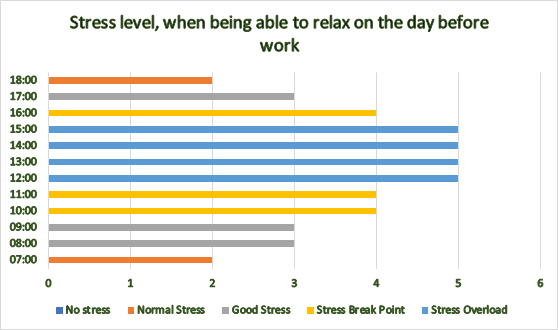
\includegraphics[width=.7\linewidth]{chap5/st1.png}
  \caption[Stress level, when being able to relax on the day before work]{Stress level, when being able to relax on the day before work\index{Hasnain}}
  \label{fig:st1}
\end{figure}

Then I checked the stress level with using Schneckenhaus system. In figure:\ref{fig:st3} shows the chart of stress level after using Schneckenhaus system with taking relax the day before work.
\begin{figure}[ht] 
  \centering
  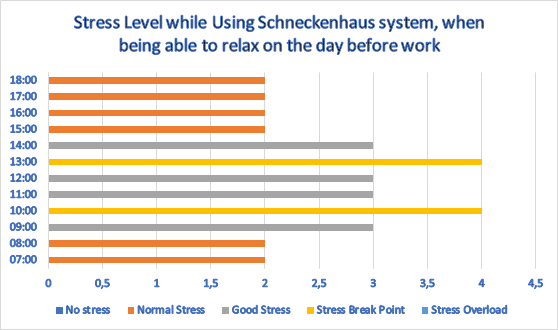
\includegraphics[width=.8\linewidth]{chap5/st3.png}
  \caption[Stress Level while Using Schneckenhaus system, when being able to relax on the day before work
]{Stress Level while Using Schneckenhaus system, when being able to relax on the day before work
\index{Hasnain}}
  \label{fig:st3}
\end{figure}
\subsubsection*{Daylong Stress level, when \textbf{not} being able to relax on the day before work}
In this condition firstly I checked stress level without using my system. In figure:\ref{fig:st2} shows the chart current stress level without taking relax day before work.
\begin{figure}[ht] 
  \centering
  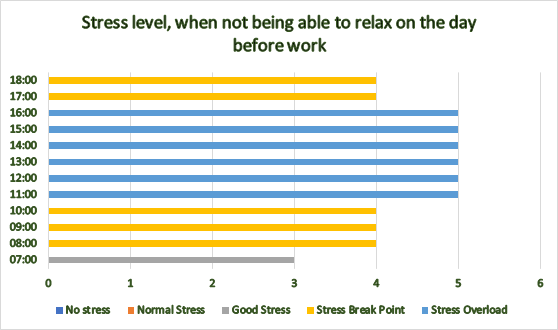
\includegraphics[width=.9\linewidth]{chap5/st2.png}
  \caption[Stress level, when not being able to relax on the day before work]{Stress level, when not being able to relax on the day before work\index{Hasnain}}
  \label{fig:st2}
\end{figure}
Then I checked stress level with using Schneckenhaus system. In figure:\ref{fig:st4} shows the chart stress level after using Schneckenhaus system without taking relax day before work.
\begin{figure}[h] 
  \centering
  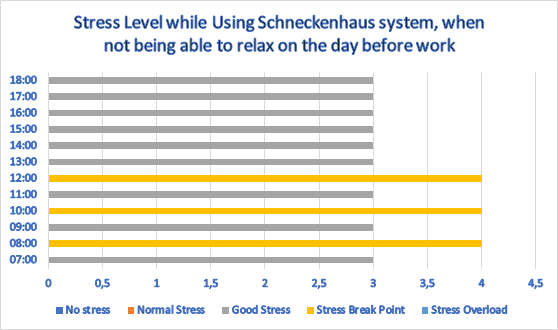
\includegraphics[width=.8\linewidth]{chap5/st4.png}
  \caption[Stress Level while Using Schneckenhaus system, when not being able to relax on the day before work
]{Stress Level while Using Schneckenhaus system, when not being able to relax on the day before work
\index{Hasnain}}
  \label{fig:st4}
\end{figure}

Based on this I found present daylong stress condition of participants and using stress management system at working condition, stress level dramatically changes on the result. The result shows that, before using Schneckenhaus system, the stress level is not controlled and unpredictable. when he starts using Schneckenhaus system, participants feel more confidante and stress level is most of the time manageable. Which is helpful for my target group, people with stress overflow at their workplace environment. 

\subsection{Jan's Feedback on Experiment}
After this experiment, our participant Jan gives his feedback regarding our solution approach and prototype. Jan said:

"In regards to the whole "Schneckenhaus"-ensemble, I think here are the reasons how it will be helpful to achieve more workplace accessibility for me:

- I think the different devices will be working as conversational "ice breakers". When we talk about Illnesses, there is a lot of anxiety on how to approach the subject and to not ask insensitive questions or not wanting to talk about private medical history. This anxiety can lead to a kind of silence around the subject that isn't very productive for anyone involved. But with the "Schneckenhaus"-ensemble I can show future bosses and colleagues there cool design and different functions and this can start a good conversation on how to achieve good workplace accessibility and teamwork.

- the light-up display will then be a next step on having good communications between me and my colleagues. Because stress sometimes makes it hard for me to speak and process conversations, it is a huge help for me to have a non-verbal communication device. It will also be helpful to my colleagues because they will know that I can't talk at the moment and won't be confused by my behaviour.

- and the chatbot with experimental sensors will be a huge help to me, to get a better overview when I should take a break and what kind of break is use full for me in a given situation. That kind of long term assistance is really helpful for me, to make the whole "taking a break for anxiety reasons" situation less awkward for me and to become more confident in my disability. Which of course means when I'm more confident I can also communicate better to my colleagues what my deal is and there will be less confusion about what is going on with me.

In short: I think the "Schneckenhaus"-ensemble will be a huge help in making future workplaces more accessible for me because it reduces confusion for my colleagues, therefore reduces stress that miscommunications might cause. And it helps me to catalogue my anxiety/break needs, therefore it helps me to become more confident in knowing my limits and taking breaks at the right time which leads to improving the quality of my work and my health."



